\documentclass[twocolumn]{article}
\usepackage[spanish]{babel}
\usepackage{caption}
\usepackage{graphicx}
\usepackage{amsmath}
\setlength{\parindent}{0pt}

\author{Josué Villasante}
\title{Potencia de un laser en función del grado de polarización}

\begin{document}
	\maketitle

	\section{Procedimiento}

		El haz de luz producido por el laser era polarizado, y tuvo una potencia de 100mW y una longitud de onda de 405nm. Este fue reflejado 90 grados primero en un cubreobjetos y luego 90 grados en un espejo. El cubreobjetos permitió reducir la potencia del haz de luz a una aceptable por el medidor, pero produjo dos haces debido a que ambas superficies reflejan. Para eliminar uno de los haces de luz más adelante se utilizó un iris. Luego se colocó el polarizador y finalmente el medidor de potencia. El polarizador utilizado fue de tipo "wire grid".

		\begin{center}
			\includegraphics[width=150pt]{img/experiment_layout.pdf}
			\captionof{figure}{Esquemática del experimento}
		\end{center}

		Antes de iniciar las mediciones se colocó el angulo del polarizador en -90 grados y moviendo el directamente el polarizador (sin mover el angulo) fue colocado en una posición donde se observó la menor potencia. A partir de ahí se empezó a medir la potencia cada 5 grados hasta llegar a 90 grados.

	\section{Resultados}

		La máxima medición fue 2382.0 $\mu$W, la menor 33.3 $\mu$W, la desviación estándar 857.20 $\mu$W y el promedio 1183.35 $\mu$W. Tomando todos los puntos y su ángulo se obtuvo la siguiente gráfica.

		\begin{center}
			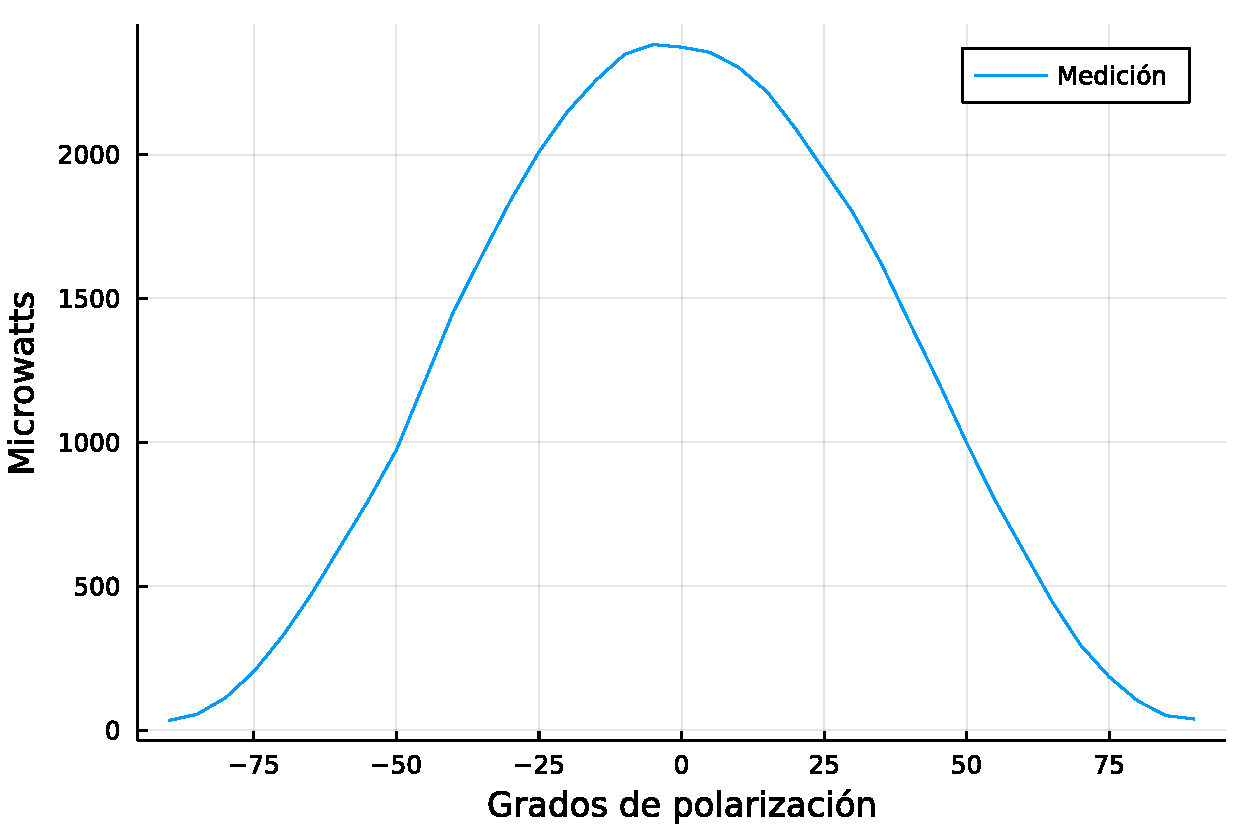
\includegraphics[width=175pt]{img/plot_raw.pdf}
			\captionof{figure}{Potencia según ángulo de polarización}
		\end{center}

	\section{Discusión}
	\subsection{Clásica}

		Una fuente de luz polarizada esta dada por
		$$
		\vec{E_p}=(\vec{E}\cdot\hat{u})\hat{u}=E_0\cos(\theta)\hat{u}
		$$

		donde $\theta$ es el angulo entre el campo eléctrico y el polarizador, y $E_0$ es la amplitud. Con esto podemos calcular la intensidad, la cual es proporcional a la potencia.

		$$
		I=|\vec E_p|^2=E_0^2\cos^2(\theta)
		$$

		Entonces las mediciones anteriores deberían se proporcionales a $\cos^2(\theta)$. Por lo tanto, comparamos los resultados con $2382\cos^2(\theta)$ y observamos que efectivamente la potencia realiza una figura muy cercana a $\cos^2(\theta)$.

		\begin{center}
			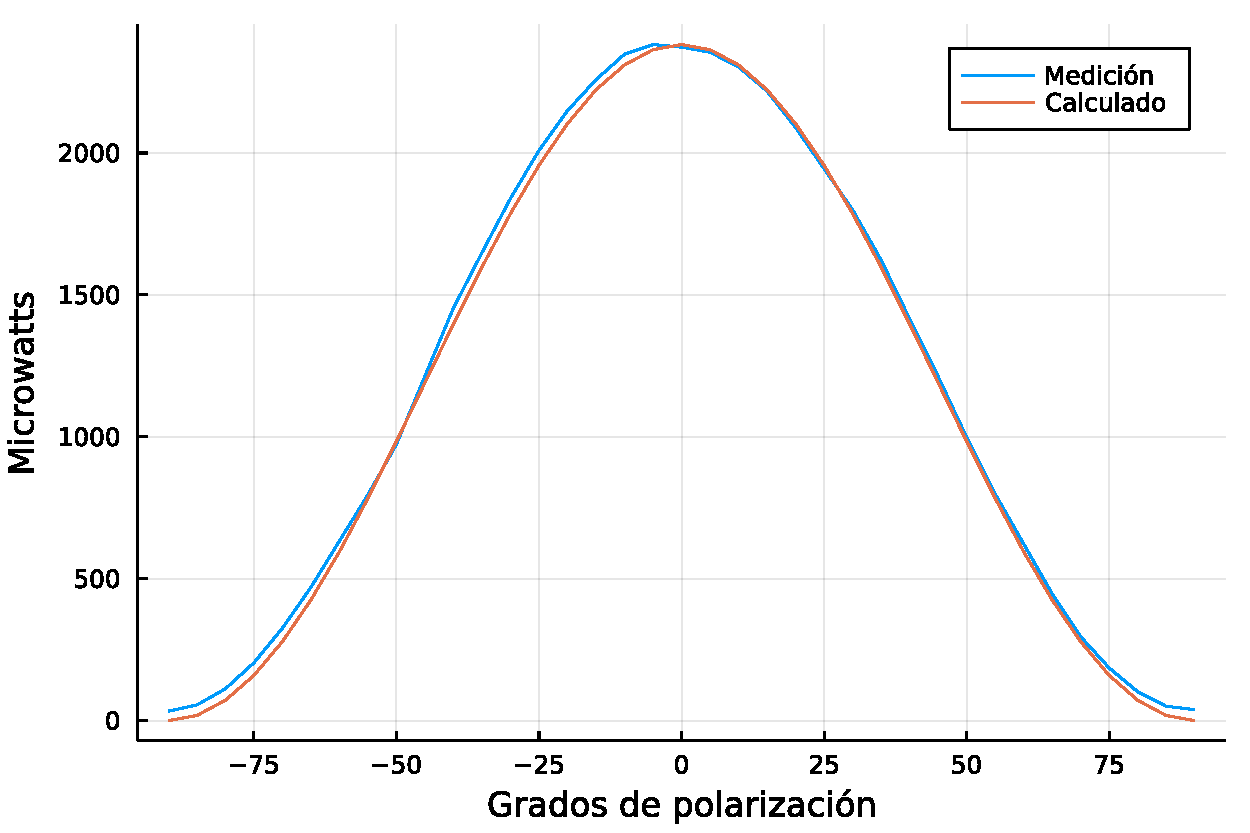
\includegraphics[width=175pt]{img/plot_compare.pdf}
			\captionof{figure}{Potencia según ángulo de polarización comparado con lo esperado}
		\end{center}
	
	\subsection{Cuántica}

		Para este caso tomamos en cuenta que inicialmente el estado del haz es

		$$
		|H\rangle
		$$

		y que luego de ser polarizado en función de $\theta$ es

		$$
		|\psi\rangle=\cos(\theta)|H\rangle+\sin(\theta)|V\rangle
		$$

		Entonces, la probabilidad de obtener un estado $|\psi\rangle$ luego de $|H\rangle$ debería proporcionar el mismo patrón que vimos anteriormente. La probabilidad está dada por

		$$
			|\langle\psi|H\rangle|^2=|\cos(\theta)\langle{H}|H\rangle + \sin(\theta)\langle{V}|H\rangle|^2
		$$
		$$
			|\langle\psi|H\rangle|^2=\cos^2(\theta)
		$$

		de manera que igualmente concuerda con los resultados obtenidos.
\end{document}